% test.tex
\subsection{Test fonctionnel}

Nous avons testé notre librairie de threads sur le programme de test
fourni et ce avec des résultats satisfaisants.

\subsection{Tests de performance}

Nous avons testé notre librairie de threads sur plusieurs cas
d'exemples, qui nous ont permis d'évaluer et de comparer pthread et
nos deux versions ; une où la run queue est décrite par une liste-fifo
et l'autre par un arbre ABR.

\subsubsection{Fibonacci}
On calcule ici le n-ième terme de la suite de Fibonacci. Pour cela un
thread appelé sur l'entier n lance 2 threads, un sur n-1, l'autre sur
n-2, les attend (join) et somme leur valeur de retour. Appelés sur 0
ou 1, les threads retournent respectivement 0 et 1.\\

Le tableau ci-dessous montre les différents résultats et temps d'exécution obtenus : \\
\begin{tabular}{|c|c|c|c|c|c|}
  \hline
  Nbre de threads & n & fibo(n)  & pthread (en micro s) & list (en micro s) & tree (en micro s)\\
  \hline
  1              & 0  & 1          &  160   & 90      & 90           \\
  32             & 5  & 8          &  650   & 160     & 160          \\
  1 024          & 10 & 89         &  8 000 & 1 150   & 1 000        \\
  32 768         & 15 & 987        &   $\infty$ & 16 000  & 11 500       \\ 
  1 048 576      & 20 & 10 946     &   $\infty$     & 165 000 & 132 000      \\
  33 554 432     & 25 & 121 393    &  $\infty$      &     $\infty$    & 1 456 000    \\
  1 073 741 824  & 30 & 1 346 269  &    $\infty$    &      $\infty$   & 16 000 000   \\
  34 359 738 368 & 35 & 14 930 352 &     $\infty$   & $\infty$        & 180 000 000  \\
\hline
\end{tabular}

\begin{center}
\rotatebox{0}{\scalebox{1}[1]{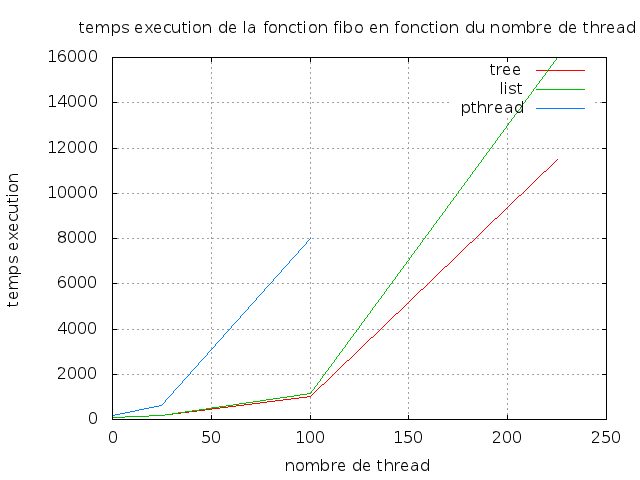
\includegraphics[width=15cm]{images/fibo.png}}}
\end{center}

\subsubsection{Somme des éléments d'un tableau}
Dans ce cas, on crée un tableau d'entiers de taille n donnée en
paramètre, on l'initialise en le remplisssant avec 0, 1, ... n-1. On
souhaite ensuite calculer la somme de ses éléments.\\ Pour ce faire,
on utilise un algoritme diviser pour régner : chaque thread appelé sur
une partie du tableau appelle deux threads, chacun appelé sur une
moitié de cette partie. Puis lorsque le thread est appelé sur un
tableau de taille 2, la somme de ces deux éléments est inscrite dans
le tableau. On obtient donc récursivement la somme de tous les
éléments du tableau.\\

Le tableau ci-dessous montre les différents résultats et temps
d'exécution obtenus : \\
\begin{tabular}{|c|c|c|c|c|c|}
  \hline Nbre de threads & n & sum(n) & pthread (en micro s) & list
  (en micro s) & tree (en micro s)\\ \hline 200 & 100 & 4 950 & 10 000
  & 1 400 & 1 000 \\ 1 000 & 500 & 124 750 & 40 000 & 9 200 & 6 000
  \\ 2 000 & 1 000 & 499 500 & 45 000 & 19 500 & 10 000 \\ 10 000 & 5
  000 & 12 497 500 & 55 000 & 85 000 & 65 000 \\ 20 000 & 10 000 & 49
  995 000 & 65 000 & 165 000 & 120 000 \\ 100 000 & 50 000 & 249 975
  000 & 75 000 & $\infty$& 600 000 \\ 200 000 & 100 000 & 704 982 704 &
  80 000 &$\infty$ & 1 200 000 \\ 1 000 000 & 500 000 & 445 698 416
  &$\infty$ &$\infty$ & 5 330 000 \\ 2 000 000 & 1 000 000 & 1 789 299 664
  &$\infty$ &$\infty$ & 10 600 000 \\ \hline
\end{tabular}

\begin{center}
\rotatebox{0}{\scalebox{1}[1]{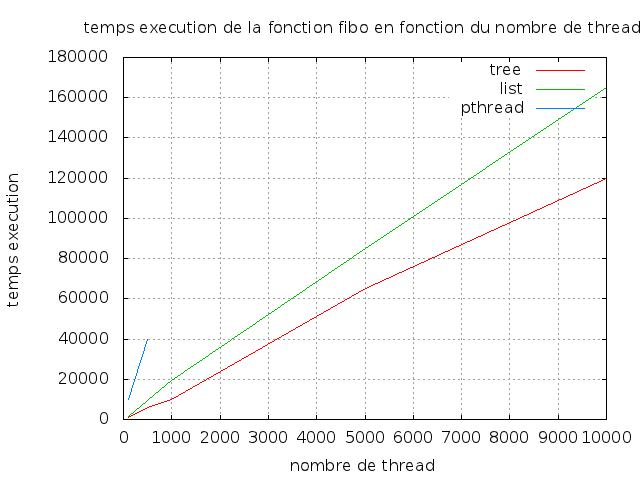
\includegraphics[width=15cm]{images/sum.png}}}
\end{center}

